\documentclass[review,authoryear]{elsarticle}

\usepackage[utf8]{inputenc}
\usepackage{amsmath,amssymb}
\usepackage{graphicx}
\usepackage{booktabs}
\usepackage{multirow}
\usepackage{siunitx}
\usepackage{natbib}

\journal{Remote Sensing of Environment}

\begin{document}

\begin{frontmatter}
\title{Supplementary Material for:\\Symbolic Regression as Spectral Feature Engineering: Discovering Interpretable Indices for Hydrothermal Alteration Mapping from Sentinel-2}
\author[citiaps]{Francisco Parra~O.}
\affiliation[citiaps]{organization={CITIAPS}, city={Santiago}, country={Chile}}
\end{frontmatter}

\setcounter{figure}{0}
\setcounter{table}{0}
\renewcommand{\thefigure}{S\arabic{figure}}
\renewcommand{\thetable}{S\arabic{table}}

\section*{Supplementary Figures}

\begin{figure*}[ht]
\centering
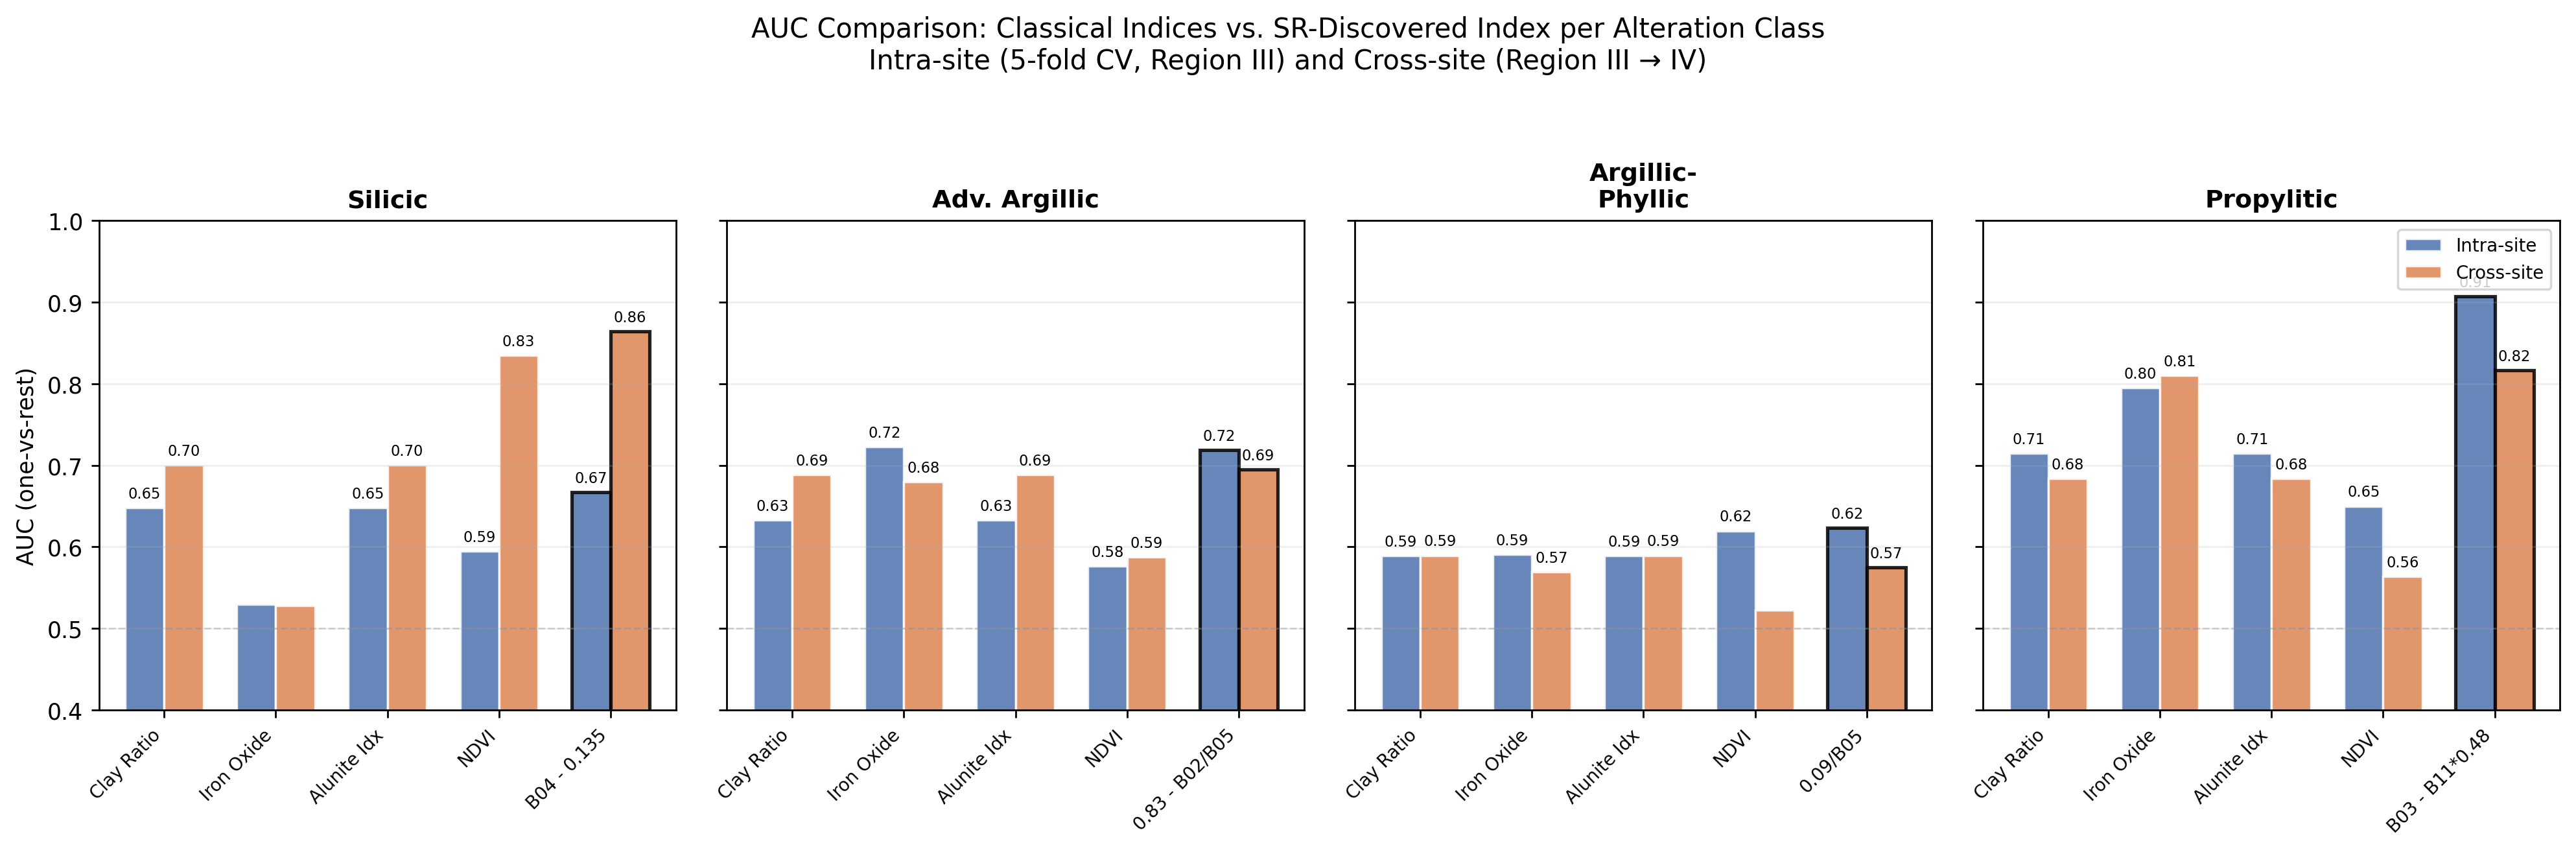
\includegraphics[width=\textwidth]{../figures/auc_comparison.png}
\caption{Per-class AUC comparison between classical indices and the corresponding SR-discovered index. Blue bars: intra-site 5-fold cross-validation (Region~III). Orange bars: cross-site validation (Region~III $\rightarrow$ Region~IV). Bold-outlined bars indicate the SR index. The dashed line at AUC = 0.5 represents random performance.}
\label{fig:s_auc_comparison}
\end{figure*}

\begin{figure*}[ht]
\centering
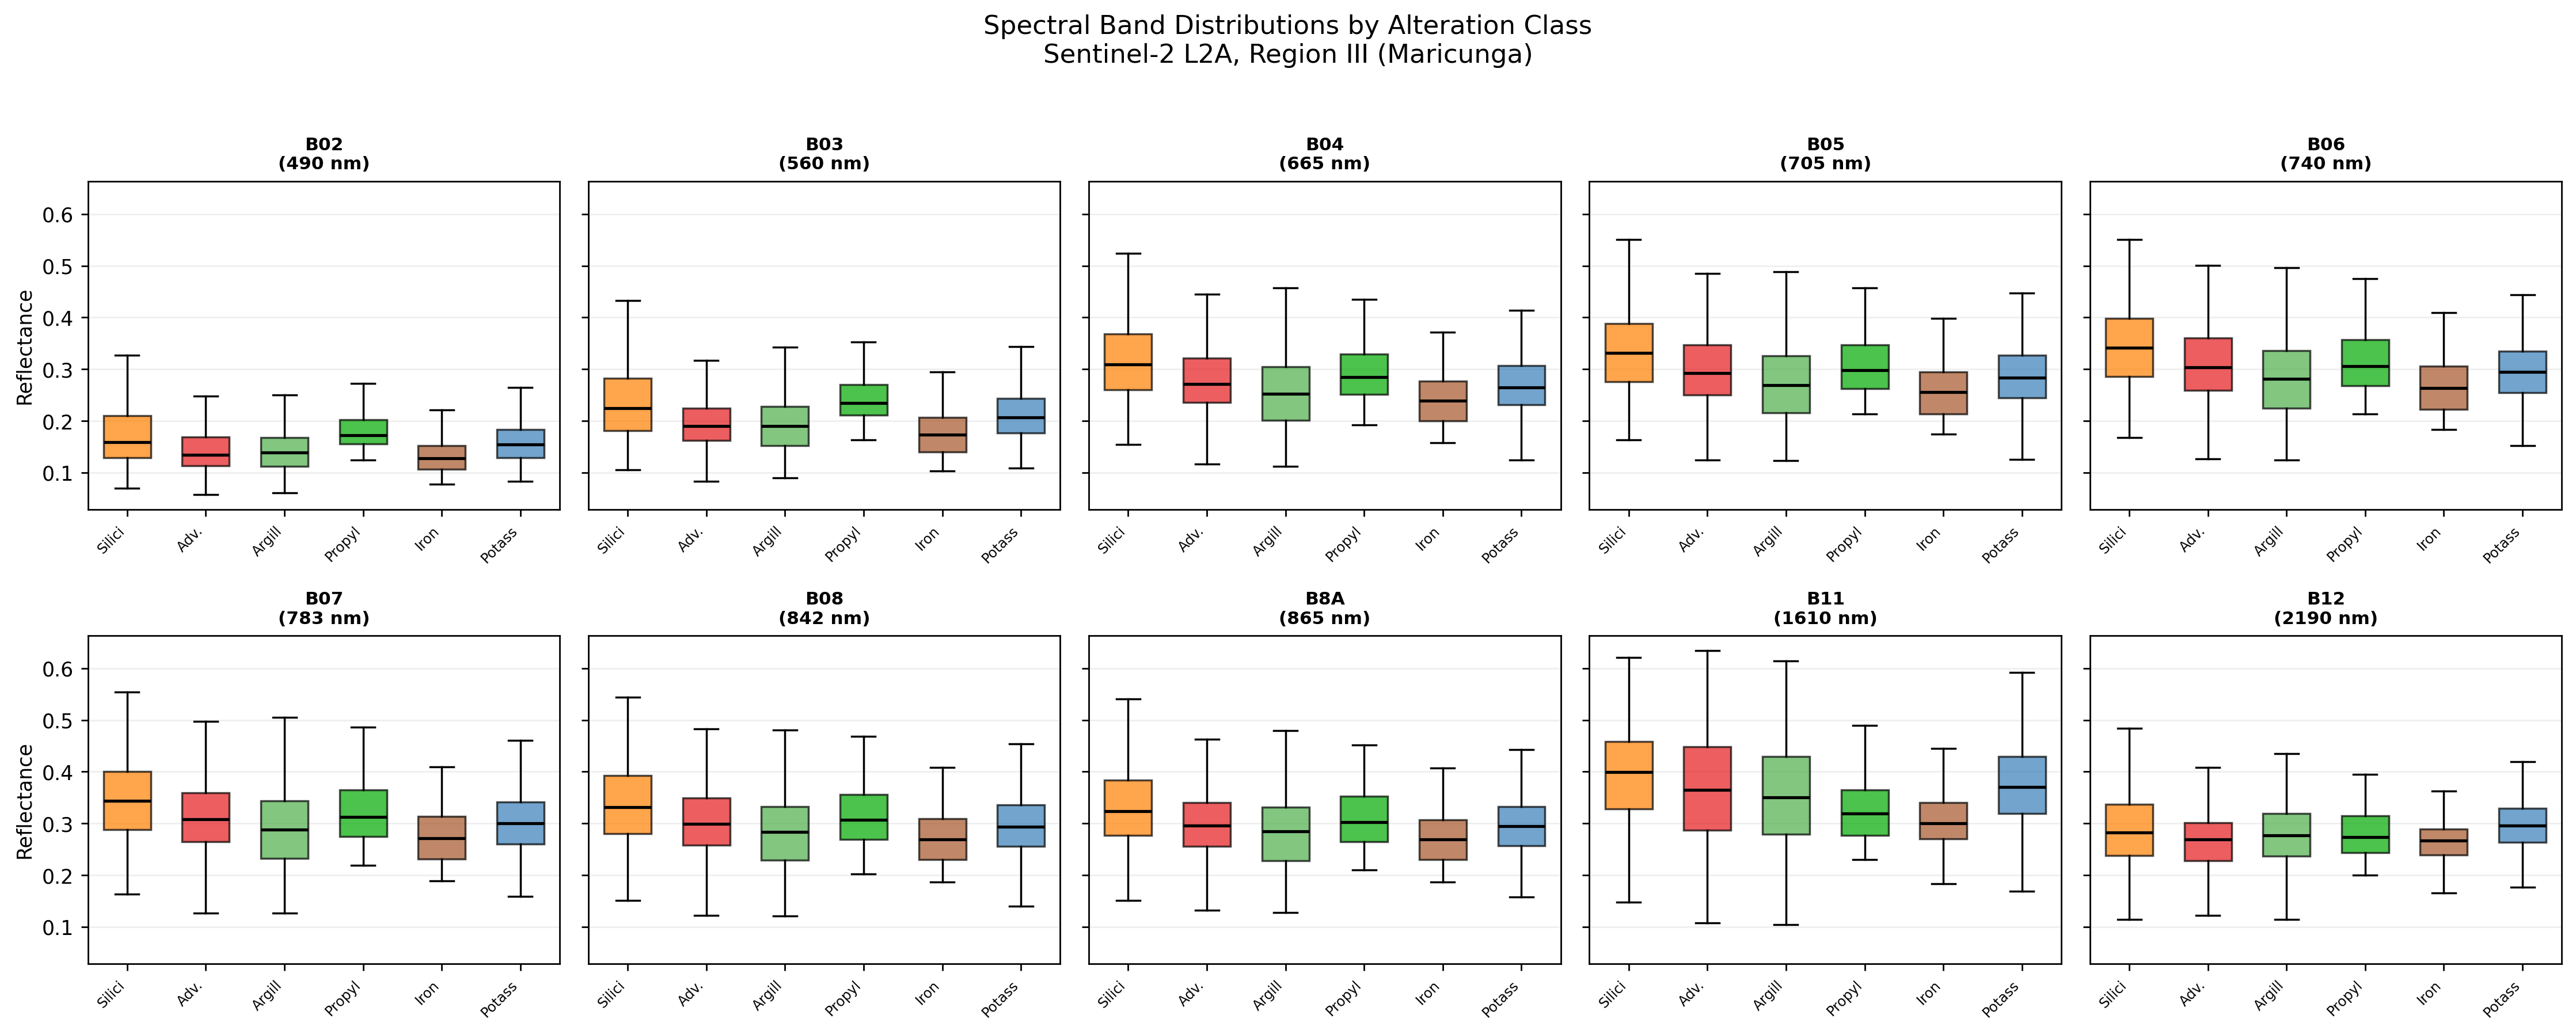
\includegraphics[width=\textwidth]{../figures/spectral_boxplots.png}
\caption{Spectral band value distributions by alteration class across all 10 Sentinel-2 bands. Boxplots show median, interquartile range, and whiskers (1.5$\times$IQR). Key discriminative bands include: B04 (Red) for silicic vs.\ other classes, B05 (Red Edge 1) for argillic types, and B11--B12 (SWIR) for propylitic and iron oxide alteration.}
\label{fig:s_boxplots}
\end{figure*}

\section*{Supplementary Tables}

\begin{table*}[ht]
\centering
\caption{Robustness check: mean AUC across alteration classes for different classifiers and feature sets (5-fold CV, Region~III). The pattern ``SR $\approx$ raw bands'' and ``SR + classical $>$ all'' is consistent across all four classifiers and two DL architectures tested.}
\label{tab:s_multiclf}
\begin{tabular}{llcccc}
\toprule
Classifier & Features & $n$ feat. & BA & Mean AUC & Best class AUC \\
\midrule
\multirow{3}{*}{RF}
  & 10 raw bands & 10 & 0.64 & 0.899 & Propyl.\ 0.99 \\
  & 6 SR indices & 6 & 0.64 & 0.898 & Propyl.\ 0.99 \\
  & 6 SR + 7 classical & 13 & 0.68 & 0.920 & Propyl.\ 1.00 \\
\midrule
\multirow{3}{*}{XGBoost}
  & 10 raw bands & 10 & 0.59 & 0.895 & Propyl.\ 0.99 \\
  & 6 SR indices & 6 & 0.60 & 0.895 & Propyl.\ 1.00 \\
  & 6 SR + 7 classical & 13 & 0.66 & 0.922 & Propyl.\ 1.00 \\
\midrule
\multirow{3}{*}{SVM-RBF}
  & 10 raw bands & 10 & 0.70 & 0.901 & Propyl.\ 1.00 \\
  & 6 SR indices & 6 & 0.69 & 0.900 & Propyl.\ 1.00 \\
  & \textbf{6 SR + 7 classical} & \textbf{13} & \textbf{0.75} & \textbf{0.926} & \textbf{Propyl.\ 1.00} \\
\midrule
\multirow{3}{*}{SVM-Linear}
  & 10 raw bands & 10 & 0.60 & 0.835 & Propyl.\ 0.99 \\
  & 6 SR indices & 6 & 0.57 & 0.813 & Propyl.\ 0.98 \\
  & 6 SR + 7 classical & 13 & 0.62 & 0.851 & Propyl.\ 1.00 \\
\midrule
\multirow{3}{*}{MLP}
  & 10 raw bands & 10 & 0.64 & 0.856 & Propyl.\ 1.00 \\
  & 6 SR indices & 6 & 0.64 & 0.859 & Propyl.\ 0.99 \\
  & 6 SR + 7 classical & 13 & 0.67 & 0.878 & Propyl.\ 1.00 \\
\midrule
\multirow{3}{*}{1D-CNN}
  & 10 raw bands & 10 & 0.52 & 0.791 & Propyl.\ 0.98 \\
  & 6 SR indices & 6 & 0.58 & 0.830 & Propyl.\ 0.99 \\
  & 6 SR + 7 classical & 13 & 0.54 & 0.792 & Propyl.\ 0.99 \\
\bottomrule
\end{tabular}
\end{table*}

\begin{table*}[ht]
\centering
\caption{Detailed per-class AUC for all classifiers and feature sets (5-fold stratified CV, intra-site Region~III). Values are mean AUC (one-versus-rest).}
\label{tab:s_multiclf_detail}
\begin{tabular}{llccccccc}
\toprule
Classifier & Features & Silicic & Adv.\ Arg. & Arg.-Ph. & Propyl. & Iron Ox. & Pot.-Sk. & Mean \\
\midrule
\multirow{3}{*}{RF}
  & 10 raw bands       & 0.862 & 0.873 & 0.841 & 0.992 & 0.937 & 0.889 & 0.899 \\
  & 6 SR indices        & 0.857 & 0.868 & 0.832 & 0.994 & 0.955 & 0.880 & 0.898 \\
  & 6 SR + 7 classical  & 0.889 & 0.891 & 0.870 & 0.995 & 0.964 & 0.908 & 0.920 \\
\midrule
\multirow{3}{*}{XGBoost}
  & 10 raw bands       & 0.852 & 0.869 & 0.833 & 0.993 & 0.943 & 0.881 & 0.895 \\
  & 6 SR indices        & 0.851 & 0.865 & 0.827 & 0.995 & 0.955 & 0.879 & 0.895 \\
  & 6 SR + 7 classical  & 0.892 & 0.897 & 0.869 & 0.997 & 0.966 & 0.909 & 0.922 \\
\midrule
\multirow{3}{*}{SVM-RBF}
  & 10 raw bands       & 0.864 & 0.873 & 0.823 & 0.998 & 0.955 & 0.890 & 0.901 \\
  & 6 SR indices        & 0.862 & 0.867 & 0.823 & 0.995 & 0.962 & 0.892 & 0.900 \\
  & \textbf{6 SR + 7 classical}  & \textbf{0.900} & \textbf{0.899} & \textbf{0.867} & \textbf{0.998} & \textbf{0.972} & \textbf{0.921} & \textbf{0.926} \\
\midrule
\multirow{3}{*}{SVM-Linear}
  & 10 raw bands       & 0.759 & 0.822 & 0.731 & 0.994 & 0.880 & 0.823 & 0.835 \\
  & 6 SR indices        & 0.745 & 0.782 & 0.692 & 0.978 & 0.861 & 0.821 & 0.813 \\
  & 6 SR + 7 classical  & 0.781 & 0.827 & 0.744 & 0.996 & 0.921 & 0.840 & 0.851 \\
\bottomrule
\end{tabular}
\end{table*}

\begin{table*}[ht]
\centering
\caption{Correlation matrix: absolute Pearson $|r|$ between SR-discovered indices and raw Sentinel-2 bands. Values $|r| > 0.70$ are in bold. Only B12 (SWIR2) has $|r| < 0.70$ with all SR indices, explaining the minimal information gain from adding raw bands to the SR feature set.}
\label{tab:s_correlation}
\begin{tabular}{lcccccccccc}
\toprule
SR Index & B02 & B03 & B04 & B05 & B06 & B07 & B08 & B8A & B11 & B12 \\
\midrule
Silicic       & \textbf{0.87} & \textbf{0.94} & \textbf{1.00} & \textbf{1.00} & \textbf{0.99} & \textbf{0.99} & \textbf{0.98} & \textbf{0.82} & 0.66 & \textbf{0.97} \\
Adv.\ Argillic & 0.50 & 0.33 & 0.03 & 0.03 & 0.07 & 0.05 & 0.03 & 0.19 & 0.01 & 0.02 \\
Argillic      & \textbf{0.74} & \textbf{0.84} & \textbf{0.93} & \textbf{0.94} & \textbf{0.94} & \textbf{0.94} & \textbf{0.93} & \textbf{0.83} & 0.69 & \textbf{0.92} \\
Propylitic    & 0.68 & 0.61 & 0.40 & 0.35 & 0.31 & 0.30 & 0.31 & 0.13 & 0.05 & 0.30 \\
Iron Oxide    & 0.43 & 0.56 & \textbf{0.71} & \textbf{0.74} & \textbf{0.76} & \textbf{0.75} & \textbf{0.72} & \textbf{0.84} & 0.44 & \textbf{0.71} \\
Potassic      & 0.01 & 0.09 & 0.32 & 0.35 & 0.37 & 0.35 & 0.32 & 0.15 & 0.25 & 0.30 \\
\midrule
Max $|r|$     & \textbf{0.87} & \textbf{0.94} & \textbf{1.00} & \textbf{1.00} & \textbf{0.99} & \textbf{0.99} & \textbf{0.98} & \textbf{0.84} & 0.69 & \textbf{0.97} \\
\bottomrule
\end{tabular}
\end{table*}

\begin{table*}[ht]
\centering
\caption{DeLong test results comparing SR-discovered indices against the best-performing classical index for each alteration class (intra-site, full training set). Significance levels: $^{***}p<0.001$, $^{*}p<0.05$, n.s.\ = not significant ($p > 0.05$).}
\label{tab:s_delong}
\begin{tabular}{llllcccc}
\toprule
Target class & SR index & Classical index & AUC$_{\text{SR}}$ & AUC$_{\text{class.}}$ & $\Delta$AUC & $z$ & $p$ \\
\midrule
Propylitic & $B_{03} - 0.48 B_{11}$ & Clay Ratio & 0.907 & 0.715 & +0.192 & 34.0 & $<$0.001$^{***}$ \\
Propylitic & $B_{03} - 0.48 B_{11}$ & OH Minerals & 0.907 & 0.860 & +0.047 & 8.7 & $<$0.001$^{***}$ \\
Silicic & $B_{04} - 0.135$ & Clay Ratio & 0.667 & 0.648 & +0.019 & 2.3 & 0.020$^{*}$ \\
Adv.\ Argillic & $0.83 - B_{02}/B_{05}$ & Iron Oxide & 0.719 & 0.723 & $-$0.004 & $-$0.7 & 0.516 n.s. \\
Iron Oxide & $(\sqrt{B_{12}}-B_{11})^2$ & Clay Ratio & 0.754 & 0.737 & +0.017 & 1.2 & 0.239 n.s. \\
\bottomrule
\end{tabular}
\end{table*}

\end{document}
